\subsection{Introduction}
Many matrix operations involve computing many simpler calculations on the components of the matrix. These calculations are often independent and can be performed in parallel. A processor would compute these sequentially but a specific hardware implementation would be able to compute them in parallel. Adding hardware-based matrix operations to a processor instruction set would allow programs to reduce the number of cycles needed to get the result and so reduce the time taken. As the average clock speed of CPUs has seen very little increase since the early 2000s moving more complicated operations to hardware allows for run time to decrease without decreasing cycle time.

This project aims to develop hardware that can perform matrix operations and integrate that into the instructions of a RISK-V processor to improve the execution time of matrix-heavy programs.

\subsection{Background}
\subsubsection{FPGAs}
As this project will use a hardware implementation, a platform is needed that can allow fast development and iterations on hardware designs. An FPGA (Field Programmable Gate Array) is a semiconductor device based around a matrix of configurable logic blocks \cite{whatisanfpga}. The user can define what logic function these blocks perform and how they are connected using HDL (Hardware Description Language) programming. Hardware can be designed in HDL and constructed on the FPGA without needing to manually build the circuit.

\subsubsection{Matrix Operations}
There are four basic operations with matrices, addition, scalar multiplication, transposition and matrix multiplication. There are multiple algorithms for matrix multiplication. The naive method takes a time of $\mathcal{O}(n^{3})$. More efficient algorithms have been found such as the Refined Laser Method with a time of $\mathcal{O}(n^{2.3728596})$ \cite{alman2020refined}. However, this is a far more complicated algorithm and would only offer better efficiency for large matrices.

In the naive method, each element of the result matrices of these functions can be independently calculated allowing for parallelism. To fully utilise this all elements of the input matrices must be accessible simultaneously which limits the scalability of the input matrix size the design can handle. Block matrix multiplication can be used to split large matrices into smaller blocks that can then be calculated. This allows the hardware to be used to compute larger matrices than it can handle as long as they have a size that is a power of two. Another advantage of the naive method is that a smaller matrix can be computed as a larger matrix by filling in the extra slots with zeros and then removing them from the result.

\subsubsection{RISK-V, Rocket Chip and Chisel}
For this project, a processor is needed to integrate the matrix accelerator with. RISC-V is an open standard instruction set architecture that can be implemented in a variety of devices such as high-performance boards by SiFive and smaller microcontrollers such as Espressif's ESP32-C3. This adoption means that more software is available for the RISC-V instruction such as Debian's risk64 port. To implement a RISC-V core on an FPGA the Rocket Chip Generator will be used. This is an open-source SoC generator that produces synthesizable RTL for implementation on an FPGA. It also allows for the integration of custom accelerators as instruction set extensions \cite{rocketchip} which is needed for this project. The FPGA being used in this project should be able to run one rocket64b core.

Rocket Chip uses the Chisel HDL based on the Scala programming language. This allows for modern programming features to be used and then generate Verilog from this code. The Verilog code can then be synthesised for an FPGA.

\subsection{Literature Review}
The following is a comparison between two papers relevant to this project, Matrix Multiplication Accelerator \cite{matrix_mult_accel} and Implementation of a RISC-V Processor with Hardware Accelerator \cite{risc-v_hard_accel}.

\begin{table}[h]
	\centering
	\resizebox{\textwidth}{!}{%
		\begin{tabular}{c|c|c|}
			\cline{2-3}
			& Matrix Multiplication Accelerator                                                                                                     & \begin{tabular}[c]{@{}c@{}}Implementation of a RISC-V Processor\\ with Hardware Accelerator\end{tabular}                                                       \\ \hline
			\multicolumn{1}{|c|}{Development Board Used}                                                                      & Cyclone V - DE1-SoC with ARM Cortex-A9                                                                                                & \begin{tabular}[c]{@{}c@{}}ZedBoard with Artix-7 FPGA \\ and ARM Cortex-A9 MPCore\end{tabular}                                                                 \\ \hline
			\multicolumn{1}{|c|}{Processor Used}                                                                              & ARM Cortex-A9 HPS                                                                                                                     & \begin{tabular}[c]{@{}c@{}}PULPino (RISC-V) \\ implemented on the FPGA\end{tabular}                                                                            \\ \hline
			\multicolumn{1}{|c|}{\begin{tabular}[c]{@{}c@{}}Connection Used Between\\ Accelerator and Processor\end{tabular}} & Parallel Port on AXI bus                                                                                                              & \begin{tabular}[c]{@{}c@{}}APB bus accessible \\ as virtual memory\end{tabular}                                                                                \\ \hline
			\multicolumn{1}{|c|}{Matrix Algorithm Used}                                                                       & \begin{tabular}[c]{@{}c@{}}Naive method with two approaches, \\ register-based using parallelism \\ and 'single-threaded' memory \\ block approach with pipelining \\ and high clock speeds\end{tabular} & Naive matrix multiplication                                                                                                                                    \\ \hline
			\multicolumn{1}{|c|}{Results}                                                                                     & \begin{tabular}[c]{@{}c@{}}Higher runtime than on HPS \\ but significantly more uniform \\ distribution of results\end{tabular}       & \begin{tabular}[c]{@{}c@{}}Performance improvement by a factor of 4.5 \\ with hardware using just 124 clock cycles \\ compared to 603 in software\end{tabular} \\ \hline
		\end{tabular}%
	}
\end{table}

Implementation of a RISC-V Processor with Hardware Accelerator provided a more in-depth explanation of the project and more useful results. An instruction set extension implementation was not used due to the added complexity so a comparison with the results found in this paper may be useful. Matrix Multiplication Accelerator provided less valuable results as runtime is not as comparable when the hardware and software approaches are running a different clock speeds, 100MHz and 925MHz. It did provide an alternative design for the hardware implementation to improve scalability but block matrix multiplication can allow for the original design to computer larger matrices. 

\newpage
\subsection{Objectives}
\subsubsection{Hardware-Based Matrix Operations}
\begin{enumerate}
	\item [(Must)]  Design and implement matrix multiplication hardware that can calculate results more efficiently than software. It should work for matrices containing integers and should be able to scale to larger matrices.
	\item [(Could)] Add addition and scalar multiplication functions to the design.
	\item [(Could)] Add support for floating point values to the design.
\end{enumerate}
\subsubsection{Integration to RISC-V Core}
\begin{enumerate}
	\item [(Must)] Generate a RISC-V core and connect it to the matrix accelerator by adding new instructions to the cores instruction set.
	\item [(Must)] Develop software to allow the use of the new instructions in programs.
\end{enumerate}
\subsubsection{Comparison of Hardware Solution Against Software}
\begin{enumerate}
	\item [(Must)] Develop a program that can benchmark the use of matrix operations through software and the hardware accelerator. Run these tests and compare.
	\item [(Could)] Test and compare an implementation that uses software parallelism.
	\item [(Could)] If other matrix functions are implemented compare these to software and see if these extra functions are worth implementing.
\end{enumerate}

\newpage			
\subsection{Methodology}
To develop the matrix accelerator a plan-based methodology will be used. The structure of the accelerator will be designed before implementation and then test-driven development will be used when implementing it. It takes a long time to synthesise and generate a bitstream from HDL and can be very hard to debug hardware when it is running on an FPGA. To test more efficiently the HDL it is simulated using the tools built into Vivado for Verilog or with ChiselTest for Chisel code.

To test the performance of the accelerator a benchmark program will be needed. This should test a range of matrix sizes and if able shapes. The test should be run multiple times to find variance in results and should measure runtime and clock cycles.

\subsection{Timeline}
The planned working hours are set out in the table below giving 12 hours a week. This may change depending on what is currently being worked on.

\begin{table}[h]
	\centering
	\begin{tabular}{c|c|c|c|c|c|}
		\cline{2-6}
		& 14:00 & 15:00 & 16:00 & 17:00 & 18:00 \\ \hline
		\multicolumn{1}{|c|}{Monday}    &       &       &       &       &       \\ \hline
		\multicolumn{1}{|c|}{Tuesday}   &       &       & X     & X     & X     \\ \hline
		\multicolumn{1}{|c|}{Wednesday} &       & X     & X     & X     &       \\ \hline
		\multicolumn{1}{|c|}{Thursday}  &       & X     & X     & X     &       \\ \hline
		\multicolumn{1}{|c|}{Friday}    &       &       & X     & X     & X     \\ \hline
	\end{tabular}
\end{table}

The Gantt chart below timetables the progress towards this project. This covers all objectives that must be completed and shows deadline submissions. Additional objectives such as adding extra functionality to the accelerator can be worked if the main objective is completed and there is still allocated time left.

\begin{adjustwidth}{-\oddsidemargin-1in+1cm}{-\rightmargin}
	\centering
	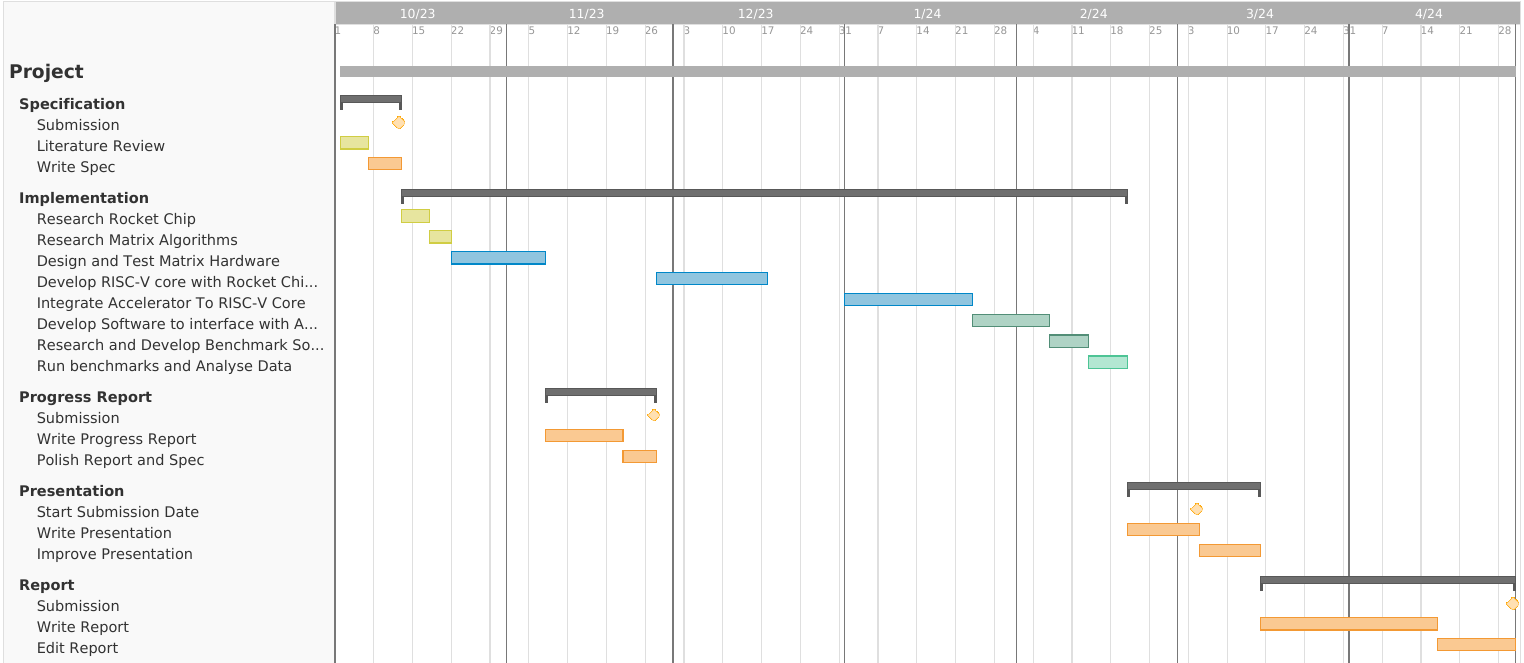
\includegraphics[width=\paperwidth-2cm, frame]{./timeline.png}
\end{adjustwidth}

\subsection{Resources}
This project will require hardware and software resources listed below as well as open-source tools such as Rocket Chip and Git.
\begin{enumerate}
	\item \textbf{FPGA Development Board - Nexys A7-100T} \newline
	This board will be used to synthesise the HDL generated by this project. It is on loan from the School of Engineering.
	\item \textbf{Vivado Design Suit} \newline
	Provides tools to synthesise and analyse HDL for FPGAs. Educational licence through the School of Engineering
	\item \textbf{vivado-risk-v project} \cite{vivado-risk-v} \newline
	An open-source project that generates RISC-V processors for FPGAs using Rocket Chip.
	\item \textbf{Linux Workstation PC} \newline
	A PC capable of running the Vivado Design Suit tools and the Ubunbtu 20.04 environment that is needed for the vivado-risk-v project. My PC fulfils these requirements.
\end{enumerate}

\subsection{Risks}
Three main risks could harm this project. These are listed below along with mitigations and solutions.
\begin{enumerate}
	\item \textbf{Damage to FPGA Development Board} \newline
	This board is on loan from the School of Engineering so a replacement could be obtained. To reduce the chance of damage the board will only be transported when necessary and kept in its protective packaging when not in use.
	\item \textbf{Damage to Workstation} \newline
	Engineering computer labs could be used to run Vivado Design Suit and DCS labs can provide a Linux environment if needed.
	\item \textbf{Data Loss} \newline
	Git version control will be used to track changes and all data relevant to the project will be backed up to GitHub providing an easy way to recover data. A log will be kept of the process to generate data such as the use of vivado-risk-v so it can be repeated if necessary.
\end{enumerate}

\subsection{Legal, Social, Ethical and Professional Issues}
This project should not present any social, ethical or professional issues and does not require working with people. There is no intent to profit from this project so no legal issues should arise. 
